\documentclass[dvisvgm]{standalone}
\usepackage{tikz}
\usetikzlibrary{patterns}

\begin{document}
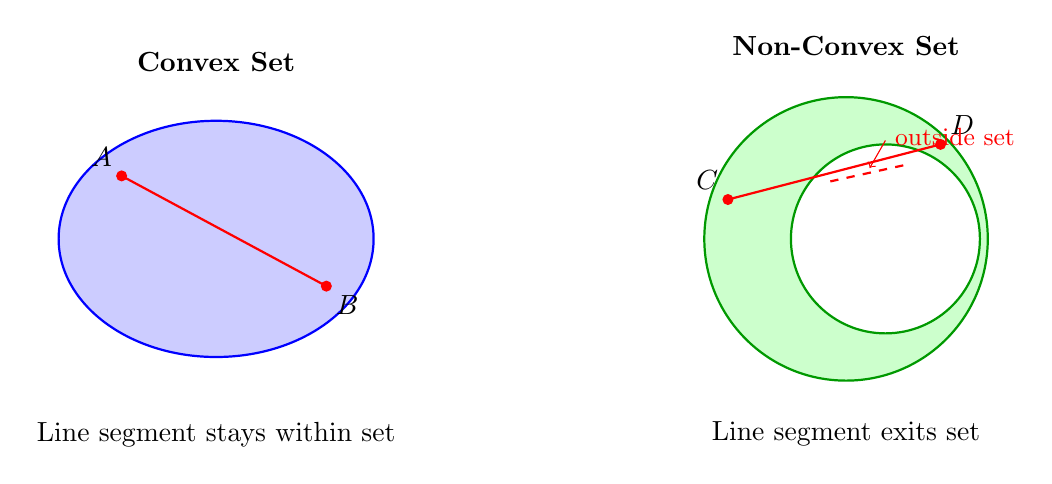
\begin{tikzpicture}

% Convex set (left side)
\begin{scope}[xshift=-4cm]
    % Draw convex set (ellipse)
    \fill[blue!20] (0,0) ellipse (2cm and 1.5cm);
    \draw[blue, thick] (0,0) ellipse (2cm and 1.5cm);
    
    % Add two points in the convex set
    \fill[red] (-1.2, 0.8) circle (2pt);
    \fill[red] (1.4, -0.6) circle (2pt);
    
    % Draw line segment between the points
    \draw[red, thick] (-1.2, 0.8) -- (1.4, -0.6);
    
    % Add labels
    \node[above] at (0, 2) {\textbf{Convex Set}};
    \node[below] at (0, -2.2) {Line segment stays within set};
    
    % Label points
    \node[above left] at (-1.2, 0.8) {$A$};
    \node[below right] at (1.4, -0.6) {$B$};
\end{scope}

% Non-convex set (right side)
\begin{scope}[xshift=4cm]
    % Draw non-convex set (crescent/moon shape)
    \fill[green!20] (0,0) circle (1.8cm);
    \fill[white] (0.5,0) circle (1.2cm);
    \draw[green!60!black, thick] (0,0) circle (1.8cm);
    \draw[green!60!black, thick] (0.5,0) circle (1.2cm);
    
    % Add two points in the non-convex set
    \fill[red] (-1.5, 0.5) circle (2pt);
    \fill[red] (1.2, 1.2) circle (2pt);
    
    % Draw line segment between the points (part goes outside)
    \draw[red, thick] (-1.5, 0.5) -- (1.2, 1.2);
    
    % Highlight the part of line that's outside the set
    \draw[red, thick, dashed] (-0.2, 0.73) -- (0.8, 0.95);
    
    % Add labels
    \node[above] at (0, 2.2) {\textbf{Non-Convex Set}};
    \node[below] at (0, -2.2) {Line segment exits set};
    
    % Label points
    \node[above left] at (-1.5, 0.5) {$C$};
    \node[above right] at (1.2, 1.2) {$D$};
    
    % Add annotation for the part outside
    \node[right, red] at (0.5, 1.3) {\small outside set};
    \draw[red, ->] (0.5, 1.25) -- (0.3, 0.9);
\end{scope}


\end{tikzpicture}
\end{document}
